\label{ap:ap11}
\chapter{Visão computacional}
\section*{\textbf{A - ENUNCIADO}}

\subsection*{\textbf{1 Extração de Características }}

\textcolor{black}{Os bancos de imagens fornecidos são conjuntos de imagens de 250x250 pixels de imuno-histoquímica
(biópsia) de câncer de mama. No total são 4 classes (0, 1+, 2+ e 3+) que estão divididas em diretórios.  O objetivo é
classificar as imagens nas categorias correspondentes. Uma base de imagens será utilizada para o treinamento e outra
para o teste do treino.}\textcolor{black}{ }

\textcolor{black}{As imagens fornecidas são recortes de uma imagem maior do tipo WSI }\textit{\textcolor{black}{(Whole
Slide Imaging}}\textcolor{black}{) disponibilizada pela Universidade de Warwick
(}\underline{\href{https://pubmed.ncbi.nlm.nih.gov/28771788/}{\textcolor{black}{link}}}\textcolor{black}{)}\textit{\textcolor{black}{.}}\textcolor{black}{ A nomenclatura das imagens
segue o padrão XX\_HER\_YYYY.png, onde XX é o número do paciente e YYYY é o número da imagem recortada. Separe a base
de treino em 80\% para treino e 20\% para validação. }\textbf{\textcolor{black}{Separe por pacientes (XX), não utilize
a separação randômica! Pois, imagens do mesmo paciente não podem estar na base de treino e de validação, pois isso pode
gerar um viés.}}\textcolor{black}{ No caso da CNN VGG16 remova a última camada de classificação e armazene os valores
da penúltima camada como um vetor de características. Após o treinamento, os modelos treinados devem ser validados na
base de teste.}\textcolor{black}{ }

\textcolor{black}{ }

%\textcolor{black}{Tarefas:}\textcolor{black}{ }
\subsubsection*{Tarefas:}

\begin{enumerate}[series=listWWNumxxiv,label=\alph*),ref=\alph*]
\item \textcolor{black}{Carregue a base de dados de }\textbf{\textcolor{black}{Treino.}}\textcolor{black}{ }
\item \textcolor{black}{Crie partições contendo 80\% para treino e 20\% para validação (atenção aos
pacientes).}\textcolor{black}{ }
\item \textcolor{black}{Extraia características utilizando LBP e a CNN VGG16 (gerando um csv para cada
extrator).}\textcolor{black}{ }
\item \textcolor{black}{Treine modelos Random Forest, SVM e RNA para predição dos dados extraídos.}\textcolor{black}{ }
\item \textcolor{black}{Carregue a base de }\textbf{\textcolor{black}{Teste }}\textcolor{black}{ e execute a tarefa 3
nesta base.}\textcolor{black}{ }
\item \textcolor{black}{Aplique os modelos treinados nos dados de treino}\textcolor{black}{ }
\item \textcolor{black}{Calcule as métricas de Sensibilidade, Especificidade e F1-Score com base em suas matrizes de
confusão.}\textcolor{black}{ }
\item \textcolor{black}{Indique qual modelo dá o melhor o resultado e a métrica utilizada}\textcolor{black}{ }
\end{enumerate}
\textcolor{black}{ }

\subsection*{\textbf{2 Redes Neurais}}

\textcolor{black}{Utilize as duas bases do exercício anterior para treinar as Redes Neurais Convolucionais VGG16 e a
Resnet50. Utilize os pesos pré-treinados (}\textit{\textcolor{black}{Transfer Learning}}\textcolor{black}{), refaça as
camadas }\textit{\textcolor{black}{Fully Connected}}\textcolor{black}{ para o problema de 4 classes. Compare os treinos
de 15 épocas com e sem }\textit{\textcolor{black}{Data Augmentation}}\textcolor{black}{. Tanto a VGG16 quanto a
Resnet50 têm como camada de entrada uma imagem 224x224x3, ou seja, uma imagem de 224x224 pixels coloridos (3 canais de
cores). Portanto, será necessário fazer uma transformação de 250x250x3 para 224x224x3. Ao fazer o
}\textit{\textcolor{black}{Data Augmentation }}\textbf{\textit{\textcolor{black}{
}}}\textbf{\textcolor{black}{ cuidado }}\textcolor{black}{ para não alterar demais as cores das imagens e atrapalhar na
classificação.}\textcolor{black}{ }

\textcolor{black}{ }

%\textcolor{black}{Tarefas:}\textcolor{black}{ }
\subsubsection*{Tarefas:}

\begin{enumerate}[series=listWWNumxxv,label=\alph*),ref=\alph*]
\item \textcolor{black}{Utilize a base de dados de }\textbf{\textcolor{black}{Treino }}\textcolor{black}{ já separadas em
treino e validação do exercício anterior}\textcolor{black}{ }
\item \textcolor{black}{Treine modelos VGG16 e Resnet50 adaptadas com e sem }\textit{\textcolor{black}{Data
Augmentation}}\textcolor{black}{ }
\item \textcolor{black}{Aplique os modelos treinados nas imagens da base de
}\textbf{\textcolor{black}{Teste}}\textcolor{black}{ }
\item \textcolor{black}{Calcule as métricas de Sensibilidade, Especificidade e F1-Score com base em suas matrizes de
confusão.}\textcolor{black}{ }
\item \textcolor{black}{Indique qual modelo dá o melhor o resultado e a métrica utilizada}\textcolor{black}{ }
\end{enumerate}
\textcolor{black}{ }

%%%%%%%%%%%%%%%%%%%%%%%%%%%%%%%%%%%%%%%%%%%%%%%%%%%%%%%%%%%%%%%%%%%%%%%%%%%%%%%%%%%%%%%%%%%%%
\section*{\textbf{B - RESOLUÇÃO}}
\subsection*{\textbf{1 Extração de Características }}
\subsubsection*{Importação das bibliotecas utilizadas}
\begin{lstlisting}[language=Python, style=input]
#Resolvendo problema compatibilidade ImageDataGenerator
!pip uninstall -y tensorflow
!pip uninstall -y tf-keras
%pip install tensorflow==2.15

import os
import random
import shutil
import csv
from collections import defaultdict
from pathlib import Path

import numpy as np
import pandas as pd
import cv2

# Keras e TensorFlow
from keras.models import Model, Sequential
from keras.layers import Dense, Dropout, Flatten
from keras.optimizers import Adam
from keras.utils import to_categorical
from keras.callbacks import ModelCheckpoint, EarlyStopping

from tensorflow.keras.applications import VGG16, ResNet50
from tensorflow.keras.preprocessing.image import ImageDataGenerator
from tensorflow.keras.applications.vgg16 import preprocess_input
from tensorflow.keras.models import load_model
from tensorflow.keras.preprocessing import image_dataset_from_directory

# Scikit-learn
from sklearn.ensemble import RandomForestClassifier
from sklearn.svm import SVC
from sklearn.model_selection import train_test_split
from sklearn.preprocessing import LabelEncoder
from sklearn.metrics import confusion_matrix, classification_report, recall_score, precision_score, f1_score

#Selecione a T4 GPU
\end{lstlisting}


\subsubsection*{Extração de Características}
\subsubsubsection*{1 Carregue a base de dados de Treino}

\begin{lstlisting}[language=Python, style=input]
!unzip Train_Warwick.zip

diretorio_dataset = '/content/Train_4cls_amostra'

dataset_treino = image_dataset_from_directory(
    diretorio_dataset,
    image_size=(250, 250),  # Tamanho das imagens
    batch_size=32,          # Tamanho do lote
    label_mode='int',      # Modo de rotulagem (inteiro)
    seed=123,              # Semente para aleatoriedade
    shuffle=True           # Aleatorizar as imagens
)

nomes_classes = dataset_treino.class_names
print("Classes:", nomes_classes)
\end{lstlisting}

\begin{lstlisting}[language=, style=output]
Found 593 files belonging to 4 classes.
Classes: ['0', '1', '2', '3']
\end{lstlisting}


\subsubsubsection*{2 Crie partições contendo 80\% para treino e 20\% para validação (atenção aos pacientes)}


\begin{lstlisting}[language=Python, style=input]
diretorio_dataset = '/content/Train_4cls_amostra'
diretorio_treino = '/content/Train_split'
diretorio_validacao = '/content/Val_split'

def remover_diretorio(caminho_dir):
    if os.path.exists(caminho_dir):
        shutil.rmtree(caminho_dir)

remover_diretorio(diretorio_treino)
remover_diretorio(diretorio_validacao)
os.makedirs(diretorio_treino, exist_ok=True)
os.makedirs(diretorio_validacao, exist_ok=True)

imagens_pacientes = defaultdict(list)
pacientes_por_classe = defaultdict(set)
for class_dir in os.listdir(diretorio_dataset):
    caminho_classe = os.path.join(diretorio_dataset, class_dir)
    if os.path.isdir(caminho_classe):
        for nome_img in os.listdir(caminho_classe):
            id_paciente = nome_img.split('_')[0]  # ID do paciente
            imagens_pacientes[id_paciente].append((os.path.join(caminho_classe, nome_img), class_dir))
            pacientes_por_classe[class_dir].add(id_paciente)

pacientes_treino = set()
pacientes_validacao = set()
for nome_classe, pacientes in pacientes_por_classe.items():
    paciente_validacao = random.choice(list(pacientes))
    pacientes_validacao.add(paciente_validacao)
    pacientes.remove(paciente_validacao)

todos_pacientes = list(imagens_pacientes.keys())
random.shuffle(todos_pacientes)

for id_paciente in todos_pacientes:
    if id_paciente not in pacientes_validacao:
        pacientes_treino.add(id_paciente)

for class_dir in os.listdir(diretorio_dataset):
    os.makedirs(os.path.join(diretorio_treino, class_dir), exist_ok=True)
    os.makedirs(os.path.join(diretorio_validacao, class_dir), exist_ok=True)

for id_paciente in pacientes_treino:
    for caminho_img, class_dir in imagens_pacientes[id_paciente]:
        shutil.move(caminho_img, os.path.join(diretorio_treino, class_dir, os.path.basename(caminho_img)))

for id_paciente in pacientes_validacao:
    for caminho_img, class_dir in imagens_pacientes[id_paciente]:
        shutil.move(caminho_img, os.path.join(diretorio_validacao, class_dir, os.path.basename(caminho_img)))

# Caminhos das pastas de treino e validação
train_dir = '/content/Train_split'
val_dir = '/content/Val_split'

def count_classes_in_directory(directory):
    class_counts = {}
    for class_folder in os.listdir(directory):
        class_path = os.path.join(directory, class_folder)
        if os.path.isdir(class_path):
            class_counts[class_folder] = len(os.listdir(class_path))
    return class_counts

# Contagem de classes na base de treino e validação
train_class_counts = count_classes_in_directory(train_dir)
val_class_counts = count_classes_in_directory(val_dir)

print("Classes treino:")
for cls, count in train_class_counts.items():
    print(f"Classe {cls}: {count} imagens")

print("\nClasses validacao:")
for cls, count in val_class_counts.items():
    print(f"Classe {cls}: {count} imagens")
\end{lstlisting}

\begin{lstlisting}[language=, style=output]
Classes treino:
Classe 1: 120 imagens
Classe 3: 120 imagens
Classe 2: 120 imagens
Classe 0: 116 imagens

Classes validacao:
Classe 1: 27 imagens
Classe 3: 30 imagens
Classe 2: 30 imagens
Classe 0: 30 imagens
\end{lstlisting}

\subsubsubsection*{3 Extraia características utilizando LBP e a CNN VGG16 (gerando um csv para cada extrator)}
%subsubsubsubsection
\subsubsubsection*{3.1 LBP}
%subsubsubsubsection

\begin{lstlisting}[language=Python, style=input]
# Função para calcular LBP
def get_pixel(img, center, x, y):
    new_value = 0
    try:
        if img[x][y] >= center:
            new_value = 1
    except:
        pass
    return new_value

def lbp_calculated_image(img):
    height, width = img.shape
    img_lbp = np.zeros((height, width), np.uint8)

    for x in range(1, height-1):
        for y in range(1, width-1):
            center = img[x][y]
            val_ar = [
                get_pixel(img, center, x-1, y-1),
                get_pixel(img, center, x-1, y),
                get_pixel(img, center, x-1, y+1),
                get_pixel(img, center, x, y+1),
                get_pixel(img, center, x+1, y+1),
                get_pixel(img, center, x+1, y),
                get_pixel(img, center, x+1, y-1),
                get_pixel(img, center, x, y-1)
            ]
            power_val = [1, 2, 4, 8, 16, 32, 64, 128]
            img_lbp[x, y] = sum(val_ar[i] * power_val[i] for i in range(len(val_ar)))

    return img_lbp

def processar_imagens(diretorio, nome_arquivo):
    caracteristicas = []

    for class_dir in os.listdir(diretorio):
        caminho_classe = os.path.join(diretorio, class_dir)
        if os.path.isdir(caminho_classe):
            for nome_img in os.listdir(caminho_classe):
                caminho_img = os.path.join(caminho_classe, nome_img)

                # Ler imagem e converter para escala de cinza
                img = cv2.imread(caminho_img, cv2.IMREAD_GRAYSCALE)

                # Calcular LBP
                img_lbp = lbp_calculated_image(img)

                # Calcular histograma
                hist = cv2.calcHist([img_lbp], [0], None, [256], [0, 256])
                hist_normalizado = hist.flatten() / hist.sum()  # Normalizar

                # Adicionar as características
                caracteristicas.append((class_dir, nome_img, *hist_normalizado))

    # Gerar CSV
    with open(nome_arquivo, 'w', newline='') as csv_file:
        writer = csv.writer(csv_file)
        writer.writerow(['Classe', 'Imagem'] + [f'Bin_{i}' for i in range(256)])  # Cabeçalho
        writer.writerows(caracteristicas)

# Processar diretórios de treino e validação
processar_imagens(diretorio_treino, '/content/caracteristicas_lbp_treino.csv')
processar_imagens(diretorio_validacao, '/content/caracteristicas_lbp_validacao.csv')

#CSV gerado com características LBP para treino e validação.
\end{lstlisting}

\subsubsubsection*{3.2 VGG}
%subsubsubsubsection

\begin{lstlisting}[language=Python, style=input]
from keras.preprocessing import image

# Carregar o modelo VGG16 pré-treinado
model_vgg = VGG16(weights='imagenet', include_top=False, pooling='avg')

def extrair_caracteristicas_vgg(diretorio, arquivo_saida):
    caracteristicas = []

    for class_dir in os.listdir(diretorio):
        caminho_classe = os.path.join(diretorio, class_dir)
        if os.path.isdir(caminho_classe):
            for nome_img in os.listdir(caminho_classe):
                caminho_img = os.path.join(caminho_classe, nome_img)

                # Pré-processar a imagem para VGG16
                img = image.load_img(caminho_img, target_size=(250, 250))  # Mudar para 250x250 se necessário
                img_array = image.img_to_array(img)
                img_array = np.expand_dims(img_array, axis=0)
                img_array = preprocess_input(img_array)

                # Extrair características
                features = model_vgg.predict(img_array)

                # Adicionar as características junto com a classe e nome da imagem
                caracteristicas.append((class_dir, nome_img, *features.flatten()))  # Flatten para um vetor

    # Gerar CSV
    with open(arquivo_saida, 'w', newline='') as csv_file:
        writer = csv.writer(csv_file)
        writer.writerow(['Classe', 'Imagem'] + [f'Feature_{i}' for i in range(features.shape[1])])  # Cabeçalho
        writer.writerows(caracteristicas)

# Chame a função para processar os diretórios de treino e validação
extrair_caracteristicas_vgg(diretorio_treino, '/content/caracteristicas_treino_vgg16.csv')
extrair_caracteristicas_vgg(diretorio_validacao, '/content/caracteristicas_validacao_vgg16.csv')
\end{lstlisting}


\subsubsubsection*{4 Treine modelos Random Forest, SVM e RNA para predição dos dados extraídos}
\subsubsubsection*{4.1 Random Forest}

\begin{lstlisting}[language=Python, style=input]
# características LBP
lbp_df_train = pd.read_csv('/content/caracteristicas_lbp_treino.csv')
lbp_df_val = pd.read_csv('/content/caracteristicas_lbp_validacao.csv')

# características VGG
vgg_df_train = pd.read_csv('/content/caracteristicas_treino_vgg16.csv')
vgg_df_val = pd.read_csv('/content/caracteristicas_validacao_vgg16.csv')

# Concatenar características LBP e VGG
X_train = pd.concat([lbp_df_train.drop(['Classe', 'Imagem'], axis=1),
                     vgg_df_train.drop(['Classe', 'Imagem'], axis=1)], axis=1)
y_train = lbp_df_train['Classe']

X_val = pd.concat([lbp_df_val.drop(['Classe', 'Imagem'], axis=1),
                   vgg_df_val.drop(['Classe', 'Imagem'], axis=1)], axis=1)
y_val = lbp_df_val['Classe']

# Treinar Random Forest
model_rf = RandomForestClassifier(n_estimators=100, random_state=42)
model_rf.fit(X_train, y_train)

# Fazer previsões no conjunto de validação
y_pred = model_rf.predict(X_val)

# Avaliar o modelo
conf_matrix = confusion_matrix(y_val, y_pred)
class_report = classification_report(y_val, y_pred)

print("Matriz de Confusao:\n", conf_matrix)
print("\nRelatorio de Classificacao:\n", class_report)
\end{lstlisting}

\begin{lstlisting}[language=, style=output]
Matriz de Confusao:
 [[27  1  0  0]
 [21  3  6  0]
 [ 0  5 25  0]
 [ 0  0  1 29]]

Relatorio de Classificacao:
               precision    recall  f1-score   support

           0       0.56      0.96      0.71        28
           1       0.33      0.10      0.15        30
           2       0.78      0.83      0.81        30
           3       1.00      0.97      0.98        30

    accuracy                           0.71       118
   macro avg       0.67      0.72      0.66       118
weighted avg       0.67      0.71      0.66       118
\end{lstlisting}

\subsubsubsection*{4.2 SVM}
\begin{lstlisting}[language=Python, style=input]
# Carregar os CSVs
data_lbp_train = pd.read_csv('/content/caracteristicas_lbp_treino.csv')
data_lbp_val = pd.read_csv('/content/caracteristicas_lbp_validacao.csv')
data_vgg_train = pd.read_csv('/content/caracteristicas_treino_vgg16.csv')
data_vgg_val = pd.read_csv('/content/caracteristicas_validacao_vgg16.csv')

print("Dimensões LBP Treino:", data_lbp_train.shape)
print("Dimensões VGG Treino:", data_vgg_train.shape)
print("Dimensões LBP Validação:", data_lbp_val.shape)
print("Dimensões VGG Validação:", data_vgg_val.shape)

# Concatenar características LBP e VGG
X_train = np.concatenate((data_lbp_train.iloc[:, 2:].values, data_vgg_train.iloc[:, 2:].values), axis=1)  # Todas as colunas exceto as duas primeiras
y_train = data_lbp_train['Classe'].values  # Usando as classes do LBP, que são as mesmas

X_val = np.concatenate((data_lbp_val.iloc[:, 2:].values, data_vgg_val.iloc[:, 2:].values), axis=1)  # Para o conjunto de validação
y_val = data_lbp_val['Classe'].values  # Usando as classes do LBP

# Treinar o modelo SVM
model_svm = SVC(kernel='linear', random_state=42)  # Você pode experimentar outros kernels como 'rbf'
model_svm.fit(X_train, y_train)

# Fazer previsões no conjunto de validação
y_pred = model_svm.predict(X_val)

# Avaliar o modelo
conf_matrix = confusion_matrix(y_val, y_pred)
report = classification_report(y_val, y_pred)

print("Matriz de Confusão:")
print(conf_matrix)
print("\nRelatório de Classificação:")
print(report)
\end{lstlisting}
\begin{lstlisting}[language=, style=output]
Dimensões LBP Treino: (475, 258)
Dimensões VGG Treino: (475, 514)
Dimensões LBP Validação: (118, 258)
Dimensões VGG Validação: (118, 514)
Matriz de Confusão:
[[25  3  0  0]
 [ 5 25  0  0]
 [ 0  4 26  0]
 [ 0  0  1 29]]

Relatório de Classificação:
              precision    recall  f1-score   support

           0       0.83      0.89      0.86        28
           1       0.78      0.83      0.81        30
           2       0.96      0.87      0.91        30
           3       1.00      0.97      0.98        30

    accuracy                           0.89       118
   macro avg       0.89      0.89      0.89       118
weighted avg       0.90      0.89      0.89       118
\end{lstlisting}

\subsubsubsection*{4.3 RNA}
\begin{lstlisting}[language=Python, style=input]
# características LBP
lbp_df_train = pd.read_csv('/content/caracteristicas_lbp_treino.csv')
lbp_df_val = pd.read_csv('/content/caracteristicas_lbp_validacao.csv')

# características VGG
vgg_df_train = pd.read_csv('/content/caracteristicas_treino_vgg16.csv')
vgg_df_val = pd.read_csv('/content/caracteristicas_validacao_vgg16.csv')

# Concatenar características LBP e VGG
X_train = pd.concat([lbp_df_train.drop(['Classe', 'Imagem'], axis=1),
                     vgg_df_train.drop(['Classe', 'Imagem'], axis=1)], axis=1)
y_train = lbp_df_train['Classe']

X_val = pd.concat([lbp_df_val.drop(['Classe', 'Imagem'], axis=1),
                   vgg_df_val.drop(['Classe', 'Imagem'], axis=1)], axis=1)
y_val = lbp_df_val['Classe']

label_encoder = LabelEncoder()
y_train_encoded = label_encoder.fit_transform(y_train)
y_val_encoded = label_encoder.transform(y_val)

y_train_categorical = to_categorical(y_train_encoded)
y_val_categorical = to_categorical(y_val_encoded)

# Criar o modelo da RNA
model_rna = Sequential()
model_rna.add(Dense(256, activation='relu', input_shape=(X_train.shape[1],)))  # Primeira camada oculta
model_rna.add(Dense(128, activation='relu'))  # Segunda camada oculta
model_rna.add(Dense(len(label_encoder.classes_), activation='softmax'))  # Camada de saída com softmax

# Compilar o modelo
model_rna.compile(optimizer='adam', loss='categorical_crossentropy', metrics=['accuracy'])

# Treinar o modelo
model_rna.fit(X_train, y_train_categorical, epochs=50, batch_size=32, validation_data=(X_val, y_val_categorical))

# Avaliar o modelo
loss, accuracy = model_rna.evaluate(X_val, y_val_categorical)
print(f'\nAcurácia no conjunto de validação: {accuracy:.4f}')
\end{lstlisting}
\begin{lstlisting}[language=, style=output]
#Acurácia no conjunto de validação: 0.8898
\end{lstlisting}

\subsubsubsection*{5 Carregue a base de Teste e execute a tarefa 3 nesta base}
\begin{lstlisting}[language=Python, style=input]
!unzip Test_Warwick.zip
\end{lstlisting}
\subsubsubsection*{tarefa 3}
\begin{lstlisting}[language=Python, style=input]
diretorio_teste = '/content/Test_4cl_amostra'

# LBP
processar_imagens(diretorio_teste, '/content/caracteristicas_lbp_teste.csv')
#CSV gerado com características LBP para a base de teste.

# VGG16
extrair_caracteristicas_vgg(diretorio_teste, '/content/caracteristicas_vgg16_teste.csv')
#CSV gerado com características VGG16 para a base de teste.
\end{lstlisting}

\subsubsubsection*{6 Aplique os modelos treinados nos dados de teste}
\begin{lstlisting}[language=Python, style=input]
# Carregar as características LBP e VGG da base de teste
lbp_df_test = pd.read_csv('/content/caracteristicas_lbp_teste.csv')
vgg_df_test = pd.read_csv('/content/caracteristicas_vgg16_teste.csv')

X_test = pd.concat([lbp_df_test.drop(['Classe', 'Imagem'], axis=1),
                    vgg_df_test.drop(['Classe', 'Imagem'], axis=1)], axis=1)

y_test = lbp_df_test['Classe']
\end{lstlisting}

\subsubsubsection*{6.1 Random Forest}
\begin{lstlisting}[language=Python, style=input]
# Fazer previsões no conjunto de teste com o modelo Random Forest treinado
y_pred_rf = model_rf.predict(X_test)

# Avaliar o modelo
conf_matrix_rf = confusion_matrix(y_test, y_pred_rf)
class_report_rf = classification_report(y_test, y_pred_rf)

print("Matriz de Confusão (Random Forest) no conjunto de teste:\n", conf_matrix_rf)
print("\nRelatório de Classificação (Random Forest) no conjunto de teste:\n", class_report_rf)
\end{lstlisting}
\begin{lstlisting}[language=, style=output]
Matriz de Confusão (Random Forest) no conjunto de teste:
 [[98  3  0  0]
 [16 49 25  0]
 [ 0 22 68  0]
 [ 0  0  4 86]]

Relatório de Classificação (Random Forest) no conjunto de teste:
               precision    recall  f1-score   support

           0       0.86      0.97      0.91       101
           1       0.66      0.54      0.60        90
           2       0.70      0.76      0.73        90
           3       1.00      0.96      0.98        90

    accuracy                           0.81       371
   macro avg       0.81      0.81      0.80       371
weighted avg       0.81      0.81      0.81       371
\end{lstlisting}

\subsubsubsection*{6.2 SVM}
\begin{lstlisting}[language=Python, style=input]
# Fazer previsões no conjunto de teste com o modelo SVM treinado
y_pred_svm = model_svm.predict(X_test)

# Avaliar o modelo
conf_matrix_svm = confusion_matrix(y_test, y_pred_svm)
class_report_svm = classification_report(y_test, y_pred_svm)

print("Matriz de Confusão (SVM) no conjunto de teste:\n", conf_matrix_svm)
print("\nRelatório de Classificação (SVM) no conjunto de teste:\n", class_report_svm)
\end{lstlisting}
\begin{lstlisting}[language=, style=output]
Matriz de Confusão (SVM) no conjunto de teste:
 [[87 14  0  0]
 [ 6 69 15  0]
 [ 0 20 69  1]
 [ 0  0  0 90]]

Relatório de Classificação (SVM) no conjunto de teste:
               precision    recall  f1-score   support

           0       0.94      0.86      0.90       101
           1       0.67      0.77      0.72        90
           2       0.82      0.77      0.79        90
           3       0.99      1.00      0.99        90

    accuracy                           0.85       371
   macro avg       0.85      0.85      0.85       371
weighted avg       0.86      0.85      0.85       371
\end{lstlisting}

\subsubsubsection*{6.3 RNA}
\begin{lstlisting}[language=Python, style=input]
# Fazer previsões no conjunto de teste com o modelo RNA treinado
y_pred_rna_prob = model_rna.predict(X_test)

# Converter probabilidades em rótulos de classe (pegando o índice da classe com maior probabilidade)
y_pred_rna = np.argmax(y_pred_rna_prob, axis=1)

# Avaliar o modelo
conf_matrix_rna = confusion_matrix(y_test, y_pred_rna)
class_report_rna = classification_report(y_test, y_pred_rna)

print("Matriz de Confusão (RNA) no conjunto de teste:\n", conf_matrix_rna)
print("\nRelatório de Classificação (RNA) no conjunto de teste:\n", class_report_rna)
\end{lstlisting}
\begin{lstlisting}[language=, style=output]
Matriz de Confusão (RNA) no conjunto de teste:
 [[96  5  0  0]
 [ 8 55 27  0]
 [ 0 21 66  3]
 [ 0  0  1 89]]

Relatório de Classificação (RNA) no conjunto de teste:
               precision    recall  f1-score   support

           0       0.92      0.95      0.94       101
           1       0.68      0.61      0.64        90
           2       0.70      0.73      0.72        90
           3       0.97      0.99      0.98        90

    accuracy                           0.82       371
   macro avg       0.82      0.82      0.82       371
weighted avg       0.82      0.82      0.82       371
\end{lstlisting}

\subsubsubsection*{7 Calcule as métricas de Sensibilidade, Especificidade e F1-Score com base em suas matrizes de confusão}
\begin{lstlisting}[language=Python, style=input]
# Função para calcular especificidade para múltiplas classes
def calcular_especificidade_multiclasse(conf_matrix):
    especificidades = []
    for i in range(conf_matrix.shape[0]):
        tn = conf_matrix.sum() - conf_matrix[i, :].sum() - conf_matrix[:, i].sum() + conf_matrix[i, i]
        fp = conf_matrix[:, i].sum() - conf_matrix[i, i]
        especificidades.append(tn / (tn + fp) if (tn + fp) > 0 else 0)
    return np.mean(especificidades)

# Cálculo das métricas para Random Forest
sensibilidade_rf = recall_score(y_test, y_pred_rf, average='macro')
f1_rf = f1_score(y_test, y_pred_rf, average='macro')
especificidade_rf = calcular_especificidade_multiclasse(conf_matrix_rf)

print(f"Métricas para Random Forest:")
print(f"F1-Score: {f1_rf:.4f}")
print(f"Sensibilidade: {sensibilidade_rf:.4f}")
print(f"Especificidade: {especificidade_rf:.4f}")
\end{lstlisting}
\begin{lstlisting}[language=, style=output]
Métricas para Random Forest:
F1-Score: 0.8034
Sensibilidade: 0.8065
Especificidade: 0.9371
\end{lstlisting}
\begin{lstlisting}[language=Python, style=input]
# Cálculo das métricas para SVM
sensibilidade_svm = recall_score(y_test, y_pred_svm, average='macro')
f1_svm = f1_score(y_test, y_pred_svm, average='macro')
especificidade_svm = calcular_especificidade_multiclasse(conf_matrix_svm)

print(f"\nMétricas para SVM:")
print(f"F1-Score: {f1_svm:.4f}")
print(f"Sensibilidade: {sensibilidade_svm:.4f}")
print(f"Especificidade: {especificidade_svm:.4f}")
\end{lstlisting}
\begin{lstlisting}[language=, style=output]
Métricas para SVM:
F1-Score: 0.8499
Sensibilidade: 0.8487
Especificidade: 0.9500
\end{lstlisting}
\begin{lstlisting}[language=Python, style=input]
# Cálculo das métricas para RNA
sensibilidade_rna = recall_score(y_test, y_pred_rna, average='macro')
f1_rna = f1_score(y_test, y_pred_rna, average='macro')
especificidade_rna = calcular_especificidade_multiclasse(conf_matrix_rna)

print(f"\nMétricas para RNA:")
print(f"F1-Score: {f1_rna:.4f}")
print(f"Sensibilidade: {sensibilidade_rna:.4f}")
print(f"Especificidade: {especificidade_rna:.4f}")
\end{lstlisting}
\begin{lstlisting}[language=, style=output]
Métricas para RNA:
F1-Score: 0.8188
Sensibilidade: 0.8210
Especificidade: 0.9419
\end{lstlisting}

\subsubsubsection*{8 Indique qual modelo dá o melhor o resultado e a métrica utilizada}
\noindent\textbf{RESULTADO}
\begin{itemize}
    \item F1-Score: SVM
    \item Sensibilidade: SVM
    \item Especificidade: SVM
\end{itemize}

SVM apresentou melhor resultado em todas as métricas.

A SVM se destacou como o melhor modelo. Ela apresentou métricas de desempenho superiores, incluindo uma F1-Score mais alta, sensibilidade e especificidade eficazes. A SVM se mostrou eficiente na classificação das imagens, principalmente devido à sua capacidade de lidar bem com dados de alta dimensionalidade e encontrar margens de separação mais precisas entre as classes.

Embora a RNA tenha também demonstrado bom desempenho, a SVM foi mais consistente, o que a torna a escolha ideal para essa tarefa específica.

%%%%%%%%%%%%%%%%%%%%%%%%%%%%%%%%%%%%%%%%%%%%%%%%%%%
\subsection*{\textbf{2 Redes Neurais}}
\subsubsection*{1 Utilize a base de dados de Treino já separadas em treino e validação do exercício anterior}
\subsubsection*{2 Treine modelos VGG16 e Resnet50 adaptadas com e sem Data Augmentation}
\subsubsubsection*{2.1 Sem Data Augmentation}
\begin{lstlisting}[language=Python, style=input]
!pip install livelossplot
from keras.optimizers import RMSprop
from keras.callbacks import ModelCheckpoint
from keras.models import Model
from keras.layers import Dense, Flatten
from keras.applications import VGG16, ResNet50
from livelossplot import PlotLossesKeras

# Definições de parâmetros
BATCH_SIZE = 64  # Tamanho do batch para treinamento
EPOCHS = 10      # Número de épocas para treinamento

# Carregar dados de treino sem Data Augmentation
train_datagen = ImageDataGenerator(rescale=1.0/255.0)
train_generator = train_datagen.flow_from_directory(
    'Train_split/',
    target_size=(224, 224),
    batch_size=BATCH_SIZE,
    class_mode='categorical',
)

# Carregar dados de validação sem Data Augmentation
validation_datagen = ImageDataGenerator(rescale=1.0/255.0)
validation_generator = validation_datagen.flow_from_directory(
    'Val_split/',
    target_size=(224, 224),
    batch_size=BATCH_SIZE,
    class_mode='categorical',
)

# Treinar modelo VGG16
model_vgg_without_augmentation = VGG16(input_shape=(224, 224, 3), weights='imagenet', include_top=False)  # Use o modelo pré-treinado

# Adicionar camadas próprias ao modelo VGG16
x_vgg = Flatten()(model_vgg_without_augmentation.output)
prediction_vgg = Dense(4, activation='softmax')(x_vgg)

# Criação do Objeto Modelo
model_vgg_without_augmentation = Model(inputs=model_vgg_without_augmentation.input, outputs=prediction_vgg)

# Compilar o modelo
model_vgg_without_augmentation.compile(loss='categorical_crossentropy', optimizer=RMSprop(learning_rate=0.0001), metrics=['accuracy'])

# Treinamento sem Data Augmentation
model_vgg_without_augmentation.fit(
    train_generator,
    validation_data=validation_generator,
    epochs=EPOCHS,
    callbacks=[PlotLossesKeras()]
)
\end{lstlisting}
\begin{figure}[h!]
\centering
\caption{Acurácia e perda VGG16 sem data augmentation}
\hspace*{-2cm} % shifts the image left
\adjustbox{valign=t, raise=0pt, margin*=0pt 0pt 0pt 0pt}{%
    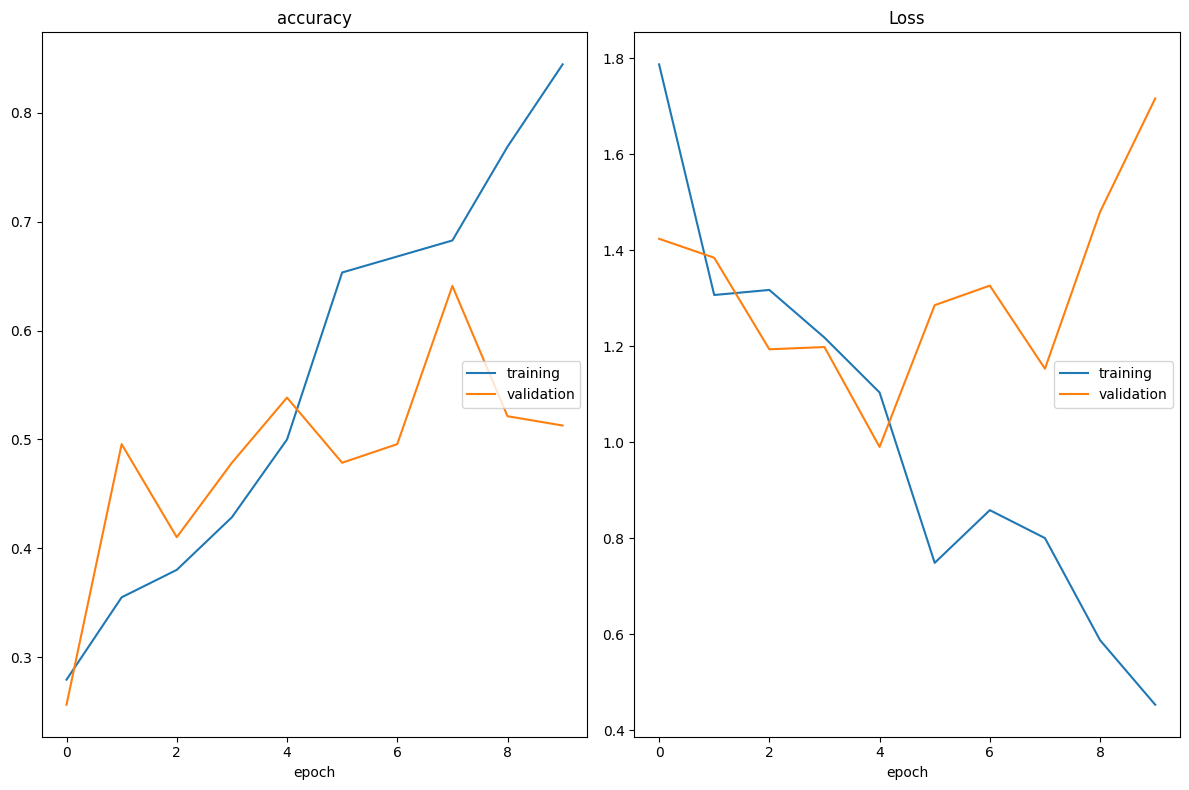
\includegraphics[width=1.2\linewidth]{apendices/fig/11_IAA011_1.png}
}
\caption*{Fonte: O autor (2025).}
\end{figure}

\begin{lstlisting}[language=, style=output]
accuracy
	training   (min: 0.279, max: 0.845, cur: 0.845)
	validation (min: 0.256, max: 0.641, cur: 0.513)
Loss
	training   (min: 0.453, max: 1.787, cur: 0.453)
	validation (min: 0.990, max: 1.716, cur: 1.716)
\end{lstlisting}


\begin{lstlisting}[language=Python, style=input]
# Treinar modelo ResNet50
model_resnet_without_augmentation = ResNet50(input_shape=(224,224,3), weights='imagenet', include_top=False)

# Não treinar os pesos existentes
for layer in model_resnet_without_augmentation.layers:
    layer.trainable = False

# Camadas próprias
x_resnet = Flatten()(model_resnet_without_augmentation.output)
prediction_resnet = Dense(4, activation='softmax')(x_resnet)

# Criação do Objeto Modelo
model_resnet_without_augmentation = Model(inputs=model_resnet_without_augmentation.input, outputs=prediction_resnet)

# Compilar o modelo
model_resnet_without_augmentation.compile(loss='categorical_crossentropy', optimizer=RMSprop(learning_rate=0.0001), metrics=['accuracy'])

# Salva o modelo Keras após cada época, porém só o de melhor resultado
checkpointer = ModelCheckpoint(filepath='img_model_no_augmentation.weights.best.keras',
                               verbose=1,
                               save_best_only=True)

# Definindo steps_per_epoch e val_steps
steps_per_epoch = train_generator.samples // BATCH_SIZE
val_steps = validation_generator.samples // BATCH_SIZE

# Treinamento sem Data Augmentation para ResNet50
model_resnet_without_augmentation.fit(
    train_generator,  # Usando o gerador de treino sem data augmentation
    epochs=EPOCHS,
    steps_per_epoch=steps_per_epoch,
    validation_data=validation_generator,
    validation_steps=val_steps,
    callbacks=[checkpointer, PlotLossesKeras()],
    verbose=False
)

print("Treinamento concluído para VGG16 e ResNet50, sem Data Augmentation.")
\end{lstlisting}
\begin{figure}[h!]
\centering
\caption{Acurácia e perda ResNet50 sem data augmentation}
\hspace*{-2cm} % shifts the image left
\adjustbox{valign=t, raise=0pt, margin*=0pt 0pt 0pt 0pt}{%
    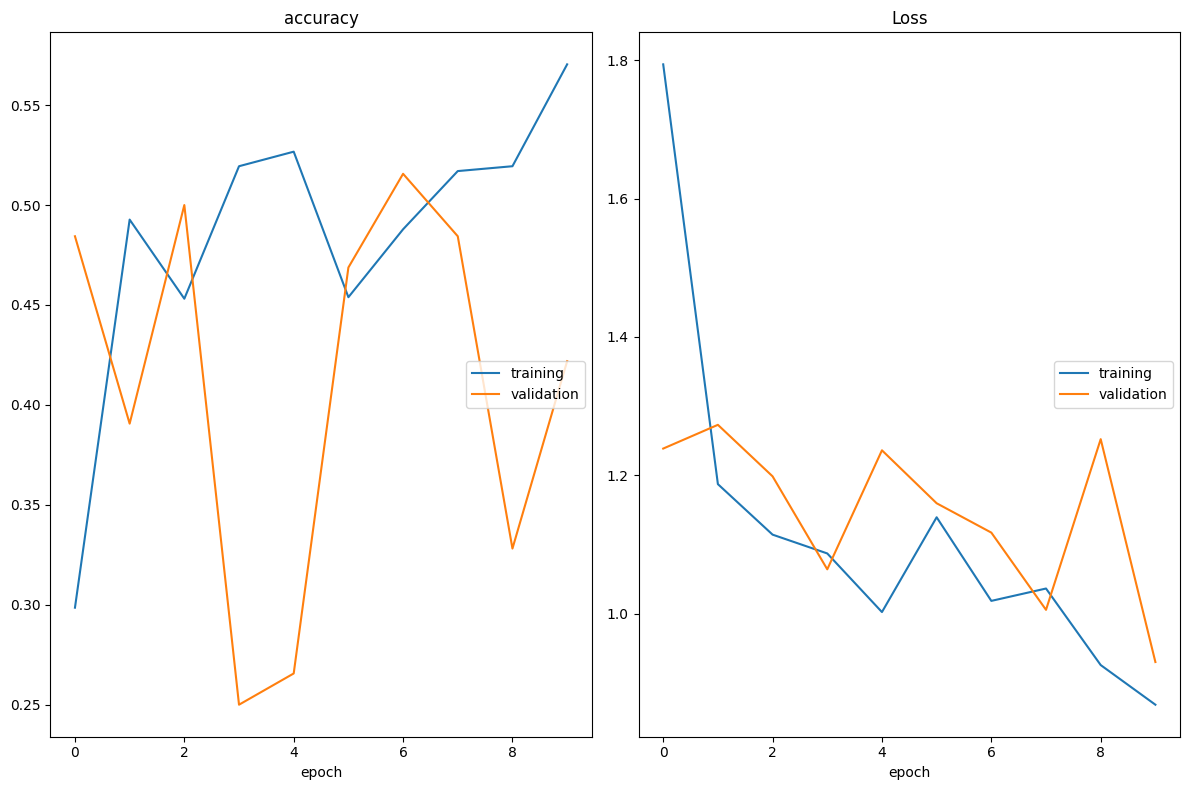
\includegraphics[width=1.2\linewidth]{apendices/fig/11_IAA011_2.png}
}
\caption*{Fonte: O autor (2025).}
\end{figure}

\begin{lstlisting}[language=, style=output]
accuracy
	training   (min: 0.299, max: 0.570, cur: 0.570)
	validation (min: 0.250, max: 0.516, cur: 0.422)
Loss
	training   (min: 0.869, max: 1.794, cur: 0.869)
	validation (min: 0.931, max: 1.273, cur: 0.931)
\end{lstlisting}


\subsubsubsection*{2.2 Com Data Augmentation}
\begin{lstlisting}[language=Python, style=input]
from keras.optimizers import RMSprop
from keras.callbacks import ModelCheckpoint
from keras.models import Model
from keras.layers import Dense, Flatten
from keras.applications import VGG16, ResNet50
from livelossplot import PlotLossesKeras
from tensorflow.keras.applications.resnet50 import preprocess_input

# Definições de parâmetros
BATCH_SIZE = 64  # Tamanho do batch para treinamento
EPOCHS = 10      # Número de épocas para treinamento

# Data Augmentation para o conjunto de treinamento
train_datagen_augmented = ImageDataGenerator(
    rescale=1.0/255.0,
    rotation_range=90,
    brightness_range=[0.1, 0.7],
    width_shift_range=0.5,
    height_shift_range=0.5,
    horizontal_flip=True,
    vertical_flip=True,
    validation_split=0.2,
    preprocessing_function=preprocess_input
)

# Carregar dados de treino com Data Augmentation
train_generator_augmented = train_datagen_augmented.flow_from_directory(
    'Train_split/',
    target_size=(224, 224),
    batch_size=BATCH_SIZE,
    class_mode='categorical',
)

# Carregar dados de validação sem Data Augmentation
validation_datagen = ImageDataGenerator(rescale=1.0/255.0, preprocessing_function=preprocess_input)
validation_generator = validation_datagen.flow_from_directory(
    'Val_split/',
    target_size=(224, 224),
    batch_size=BATCH_SIZE,
    class_mode='categorical',
)

# Treinar modelo VGG16
model_vgg_with_augmentation = VGG16(input_shape=(224, 224, 3), weights='imagenet', include_top=False)  # Use o modelo pré-treinado

# Adicionar camadas próprias ao modelo VGG16
x_vgg = Flatten()(model_vgg_with_augmentation.output)
prediction_vgg = Dense(4, activation='softmax')(x_vgg)

# Criação do Objeto Modelo
model_vgg_with_augmentation = Model(inputs=model_vgg_with_augmentation.input, outputs=prediction_vgg)

# Compilar o modelo
model_vgg_with_augmentation.compile(loss='categorical_crossentropy', optimizer=RMSprop(learning_rate=0.0001), metrics=['accuracy'])

# Treinamento com Data Augmentation
model_vgg_with_augmentation.fit(
    train_generator_augmented,
    validation_data=validation_generator,
    epochs=EPOCHS,
    callbacks=[PlotLossesKeras()]
)
\end{lstlisting}
\begin{figure}[h!]
\centering
\caption{Acurácia e perda VGG16 com data augmentation}
\hspace*{-2cm} % shifts the image left
\adjustbox{valign=t, raise=0pt, margin*=0pt 0pt 0pt 0pt}{%
    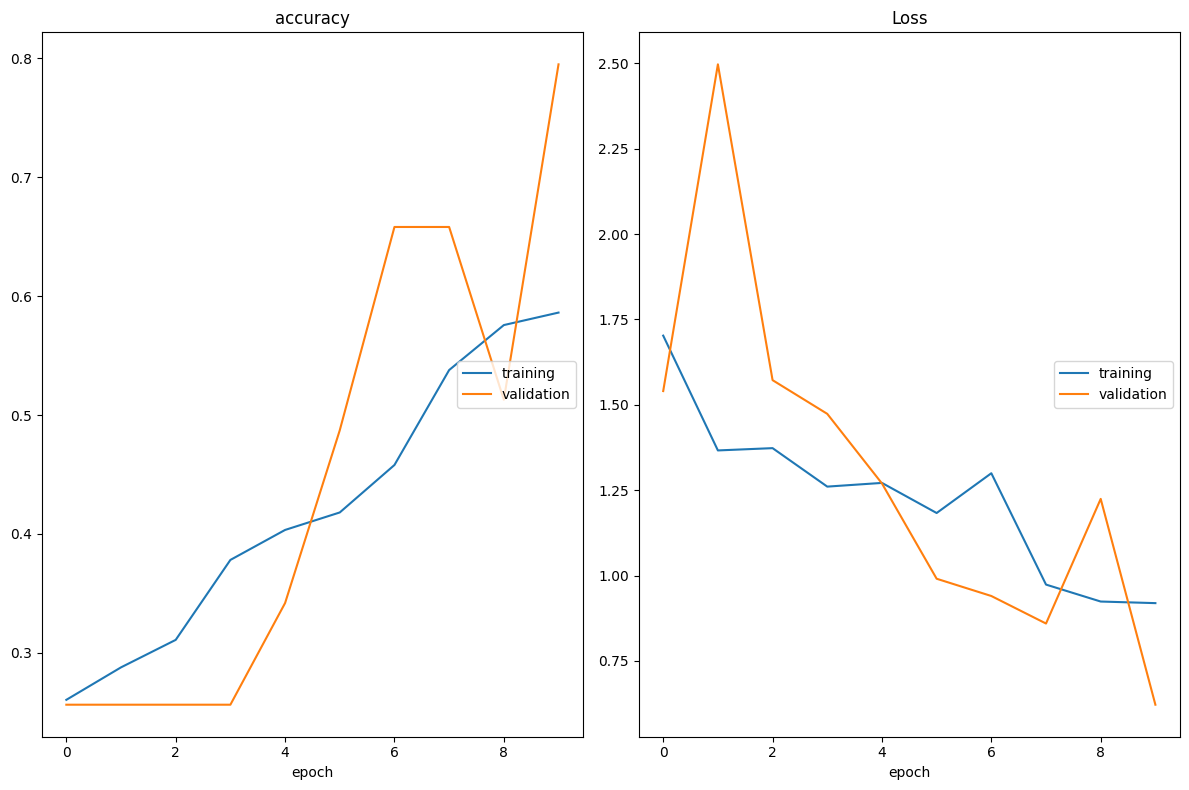
\includegraphics[width=1.2\linewidth]{apendices/fig/11_IAA011_3.png}
}
\caption*{Fonte: O autor (2025).}
\end{figure}

\begin{lstlisting}[language=, style=output]
accuracy
	training   (min: 0.261, max: 0.586, cur: 0.586)
	validation (min: 0.256, max: 0.795, cur: 0.795)
Loss
	training   (min: 0.919, max: 1.703, cur: 0.919)
	validation (min: 0.622, max: 2.497, cur: 0.622)
\end{lstlisting}


\begin{lstlisting}[language=Python, style=input]
# Treinar modelo ResNet50
model_resnet_with_augmentation = ResNet50(input_shape=(224,224,3), weights='imagenet', include_top=False)

# Não treinar os pesos existentes
for layer in model_resnet_with_augmentation.layers:
    layer.trainable = False

# Camadas próprias
x_resnet = Flatten()(model_resnet_with_augmentation.output)
prediction_resnet = Dense(4, activation='softmax')(x_resnet)

# Criação do Objeto Modelo
model_resnet_with_augmentation = Model(inputs=model_resnet_with_augmentation.input, outputs=prediction_resnet)

# Compilar o modelo
model_resnet_with_augmentation.compile(loss='categorical_crossentropy', optimizer=RMSprop(learning_rate=0.0001), metrics=['accuracy'])

# Salva o modelo Keras após cada época, porém só o de melhor resultado
checkpointer = ModelCheckpoint(filepath='img_model_tl.weights.best.keras',
                               verbose=1,
                               save_best_only=True)

# Definindo steps_per_epoch e val_steps
steps_per_epoch = train_generator_augmented.samples // BATCH_SIZE
val_steps = validation_generator.samples // BATCH_SIZE

# Treinamento com Data Augmentation para ResNet50
model_resnet_with_augmentation.fit(
    train_generator_augmented,  # Usando o gerador de treino com data augmentation
    epochs=EPOCHS,
    steps_per_epoch=steps_per_epoch,
    validation_data=validation_generator,
    validation_steps=val_steps,
    callbacks=[checkpointer, PlotLossesKeras()],
    verbose=False
)

print("Treinamento concluído para VGG16 e ResNet50, com Data Augmentation.")
\end{lstlisting}
\begin{figure}[h!]
\centering
\caption{Acurácia e perda ResNet50 com data augmentation}
\hspace*{-2cm} % shifts the image left
\adjustbox{valign=t, raise=0pt, margin*=0pt 0pt 0pt 0pt}{%
    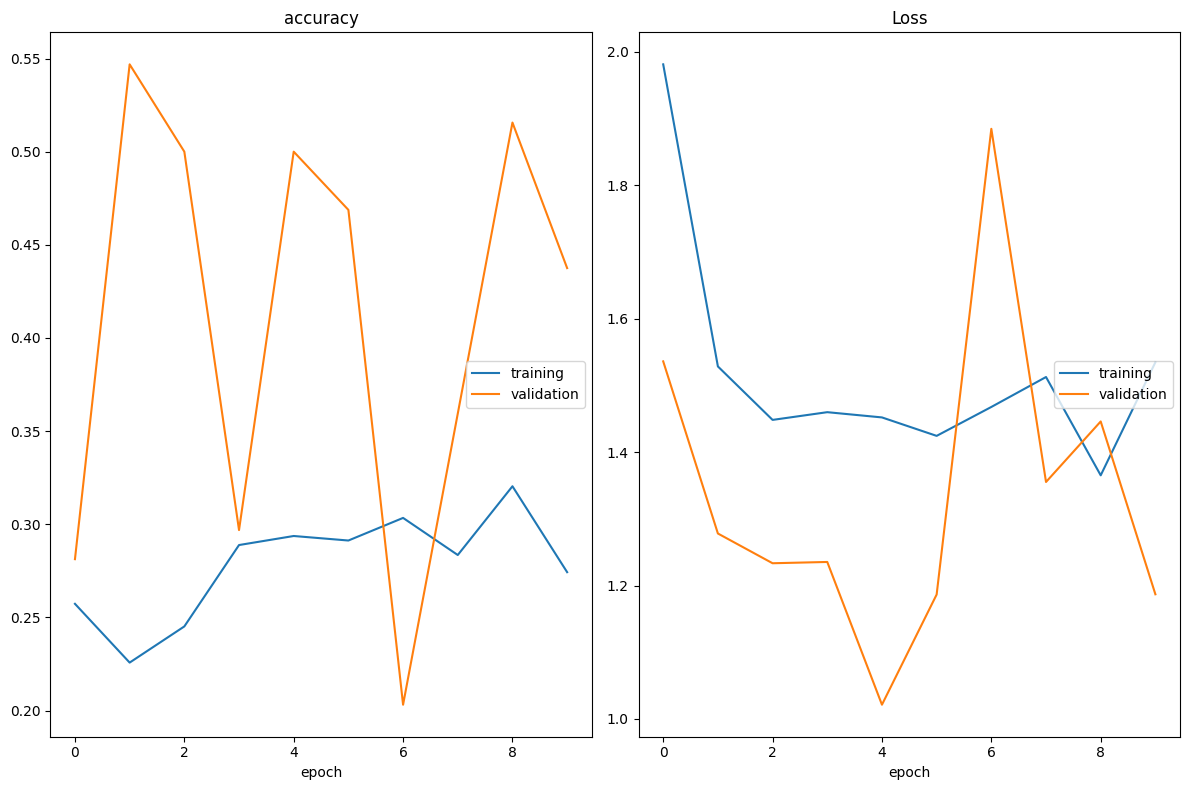
\includegraphics[width=1.2\linewidth]{apendices/fig/11_IAA011_4.png}
}
\caption*{Fonte: O autor (2025).}
\end{figure}

\begin{lstlisting}[language=, style=output]
accuracy
	training   (min: 0.226, max: 0.320, cur: 0.274)
	validation (min: 0.203, max: 0.547, cur: 0.438)
Loss
	training   (min: 1.365, max: 1.981, cur: 1.535)
	validation (min: 1.021, max: 1.884, cur: 1.187)
\end{lstlisting}


\subsubsection*{3 Aplique os modelos treinados nas imagens da base de Teste}

\begin{lstlisting}[language=Python, style=input]
test_generator = ImageDataGenerator(preprocessing_function=preprocess_input, rescale=1.0/255.0)
testgen = test_generator.flow_from_directory('/content/Test_4cl_amostra',
                                             target_size=(224, 224),
                                             batch_size=BATCH_SIZE,
                                             class_mode=None,
                                             #classes=class_subset,
                                             shuffle=False,
                                             seed=42)

test_dir = '/content/Test_4cl_amostra'

def carregar_imagens_teste(diretorio):
    imagens = []
    classes = []

    for class_dir in os.listdir(diretorio):
        caminho_classe = os.path.join(diretorio, class_dir)
        if os.path.isdir(caminho_classe):
            for nome_img in os.listdir(caminho_classe):
                caminho_img = os.path.join(caminho_classe, nome_img)

                # Ler a imagem, redimensionar e normalizar
                img = cv2.imread(caminho_img)
                img = cv2.resize(img, (224, 224))
                img = img / 255.0
                imagens.append(img)
                classes.append(int(class_dir))

    return np.array(imagens), np.array(classes)

#X_test, y_test = carregar_imagens_teste(test_dir)

# Modelos sem Data Augmentation
#y_pred_vgg16_no_aug = model_vgg_no_augmentation.predict(X_test)
y_pred_vgg16_no_aug = model_vgg_without_augmentation.predict(testgen)
y_pred_resnet50_no_aug = model_resnet_without_augmentation.predict(testgen)

# Modelos com Data Augmentation
y_pred_vgg16_aug = model_vgg_with_augmentation.predict(testgen)
y_pred_resnet50_aug = model_resnet_with_augmentation.predict(testgen)

y_pred_vgg16_no_aug_classes = np.argmax(y_pred_vgg16_no_aug, axis=1)
y_pred_resnet50_no_aug_classes = np.argmax(y_pred_resnet50_no_aug, axis=1)

y_pred_vgg16_aug_classes = np.argmax(y_pred_vgg16_aug, axis=1)
y_pred_resnet50_aug_classes = np.argmax(y_pred_resnet50_aug, axis=1)
\end{lstlisting}


\subsubsection*{4 Calcule as métricas de Sensibilidade, Especificidade e F1-Score com base em suas matrizes de confusão}

\begin{lstlisting}[language=Python, style=input]
# Cálculo das métricas para cada modelo
y_true = testgen.classes

# VGG16 sem Data Augmentation
conf_matrix_vgg16_no_aug = confusion_matrix(y_true, y_pred_vgg16_no_aug_classes)
sensibilidade_vgg16_no_aug = recall_score(y_true, y_pred_vgg16_no_aug_classes, average='macro')
f1_vgg16_no_aug = f1_score(y_true, y_pred_vgg16_no_aug_classes, average='macro')
especificidade_vgg16_no_aug = calcular_especificidade_multiclasse(conf_matrix_vgg16_no_aug)

print("Métricas VGG16 sem Data Augmentation:")
print(f"F1-Score: {f1_vgg16_no_aug:.4f}")
print(f"Sensibilidade: {sensibilidade_vgg16_no_aug:.4f}")
print(f"Especificidade: {especificidade_vgg16_no_aug:.4f}\n")

# ResNet50 sem Data Augmentation
conf_matrix_resnet50_no_aug = confusion_matrix(y_true, y_pred_resnet50_no_aug_classes)
sensibilidade_resnet50_no_aug = recall_score(y_true, y_pred_resnet50_no_aug_classes, average='macro')
f1_resnet50_no_aug = f1_score(y_true, y_pred_resnet50_no_aug_classes, average='macro')
especificidade_resnet50_no_aug = calcular_especificidade_multiclasse(conf_matrix_resnet50_no_aug)

print("Métricas ResNet50 sem Data Augmentation:")
print(f"F1-Score: {f1_resnet50_no_aug:.4f}")
print(f"Sensibilidade: {sensibilidade_resnet50_no_aug:.4f}")
print(f"Especificidade: {especificidade_resnet50_no_aug:.4f}\n")

# VGG16 com Data Augmentation
conf_matrix_vgg16_aug = confusion_matrix(y_true, y_pred_vgg16_aug_classes)
sensibilidade_vgg16_aug = recall_score(y_true, y_pred_vgg16_aug_classes, average='macro')
f1_vgg16_aug = f1_score(y_true, y_pred_vgg16_aug_classes, average='macro')
especificidade_vgg16_aug = calcular_especificidade_multiclasse(conf_matrix_vgg16_aug)

print("Métricas VGG16 com Data Augmentation:")
print(f"F1-Score: {f1_vgg16_aug:.4f}")
print(f"Sensibilidade: {sensibilidade_vgg16_aug:.4f}")
print(f"Especificidade: {especificidade_vgg16_aug:.4f}\n")

# ResNet50 com Data Augmentation
conf_matrix_resnet50_aug = confusion_matrix(y_true, y_pred_resnet50_aug_classes)
sensibilidade_resnet50_aug = recall_score(y_true, y_pred_resnet50_aug_classes, average='macro')
f1_resnet50_aug = f1_score(y_true, y_pred_resnet50_aug_classes, average='macro')
especificidade_resnet50_aug = calcular_especificidade_multiclasse(conf_matrix_resnet50_aug)

print("Métricas ResNet50 com Data Augmentation:")
print(f"F1-Score: {f1_resnet50_aug:.4f}")
print(f"Sensibilidade: {sensibilidade_resnet50_aug:.4f}")
print(f"Especificidade: {especificidade_resnet50_aug:.4f}")
\end{lstlisting}

\begin{lstlisting}[language=, style=output]
Métricas VGG16 sem Data Augmentation:
F1-Score: 0.2912
Sensibilidade: 0.3240
Especificidade: 0.7704

Métricas ResNet50 sem Data Augmentation:
F1-Score: 0.4255
Sensibilidade: 0.4898
Especificidade: 0.8316

Métricas VGG16 com Data Augmentation:
F1-Score: 0.8277
Sensibilidade: 0.8444
Especificidade: 0.9486

Métricas ResNet50 com Data Augmentation:
F1-Score: 0.3287
Sensibilidade: 0.5000
Especificidade: 0.8301
\end{lstlisting}

\subsubsection*{5 Indique qual modelo dá o melhor o resultado e a métrica utilizada}

\noindent\textbf{RESULTADO}
\begin{itemize}
    \item F1-Score: VGG16 com Data Augmentation
    \item Sensibilidade: VGG16 com Data Augmentation
    \item Especificidade: VGG16 com Data Augmentation
\end{itemize}

VGG16 com Data Augmentation apresentou melhor resultado em todas as métricas.

Após avaliar as performances dos modelos VGG16 e ResNet50 em diferentes configurações, a VGG16 com Data Augmentation se destacou como a melhor opção. Este modelo apresentou as melhores métricas de desempenho, com uma F1-Score superior, sensibilidade e especificidade elevadas.

Em contraste, a ResNet50, embora eficaz, não alcançou resultados tão robustos quanto o VGG16 em situações semelhantes. Assim, a VGG16 com Data Augmentation foi escolhida como o modelo ideal para a tarefa em questão, garantindo uma classificação mais precisa e confiável.